\section[Exact Deterministic k-NN Perturbation Criterion]{Exact Deterministic $k$-NN Perturbation Criterion}
\label{sec:knn-criterion}

Once the perturbation type is fixed, a deterministic $k$-NN prediction can only
change for one structural reason: the signed class vote inside the ordered
top-$k$ neighborhood crosses zero. This section makes that statement exact.

For an ordered sample $S$ and query $x$, let
$\pi_S^x(1),\ldots,\pi_S^x(n)$ be the sample indices sorted by increasing
distance to $x$ and then by sample index. Write
\[
N_k(S,x)=\big(\pi_S^x(1),\ldots,\pi_S^x(k)\big)
\]
for the ordered top-$k$ neighbor list and define the signed vote margin
\[
M_k(S,x)=\sum_{r=1}^k \big(2y_{\pi_S^x(r)}-1\big).
\]
Under the label-order tie-break $0 \prec 1$, the deterministic classifier
predicts label $1$ exactly when $M_k(S,x)>0$.

\begin{proposition}[Margin crossing criterion]
\label{prop:5.1}
Fix $S$, $k$, and a query $x$. Let $S'$ be any perturbed sample of the same
ambient metric space, interpreted with the same deterministic tie-breaking rule.
Then
\[
h_S^{(k)}(x)\neq h_{S'}^{(k)}(x)
\]
if and only if the signed vote margins satisfy
\[
\big(M_k(S,x)\le 0 < M_k(S',x)\big)
\quad\text{or}\quad
\big(M_k(S',x)\le 0 < M_k(S,x)\big).
\]
\end{proposition}

\begin{proof}
By definition of the deterministic vote rule, the prediction is $1$ exactly for
strictly positive signed margin and $0$ otherwise. Therefore the prediction
changes precisely when one margin is positive and the other is non-positive.
\end{proof}

\cref{prop:5.1} is elementary but useful: every perturbation
argument can be reduced to tracking how the ordered top-$k$ membership changes
and how the corresponding signed vote changes.

\begin{figure}[t]
    \centering
    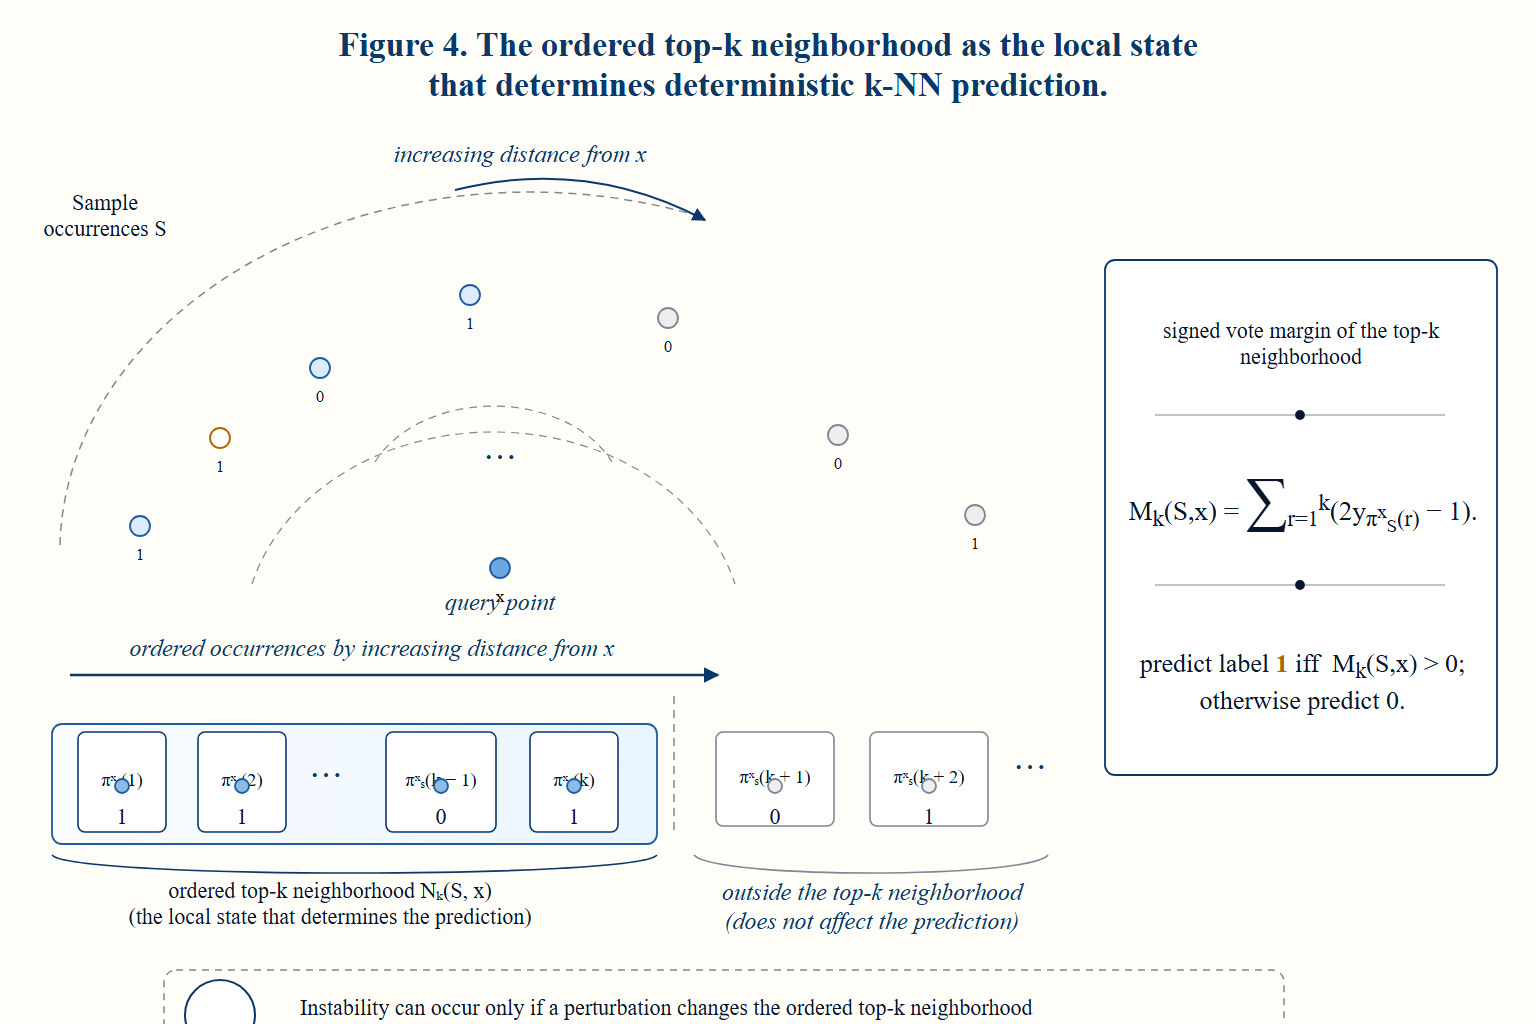
\includegraphics[width=0.82\linewidth]{outputs/figures/recreated_fig04.png}
    \caption{Ordered top-$k$ membership determines the relevant local state for
    deterministic $k$-NN. Instability is possible only when a perturbation
    changes this neighborhood or flips the labels of occurrences already inside
    it.}
    \label{fig:topk-boundary}
\end{figure}

Two immediate consequences are worth isolating. First, deleting an occurrence
outside $N_k(S,x)$ cannot change the prediction at $x$ unless the deletion also
shifts the boundary and pulls a new occurrence into the top-$k$ set
(\cref{fig:stable-deletion}, \Cref{app:additional-figures}). Second, a
replace-one perturbation can act in two different ways: it can change the
geometry of who enters the neighborhood, or it can leave the geometry fixed and
still flip the vote by changing the label attached to a strategically placed
occurrence (\cref{fig:replace-flip}, \Cref{app:additional-figures}).

\begin{figure}[t]
    \centering
    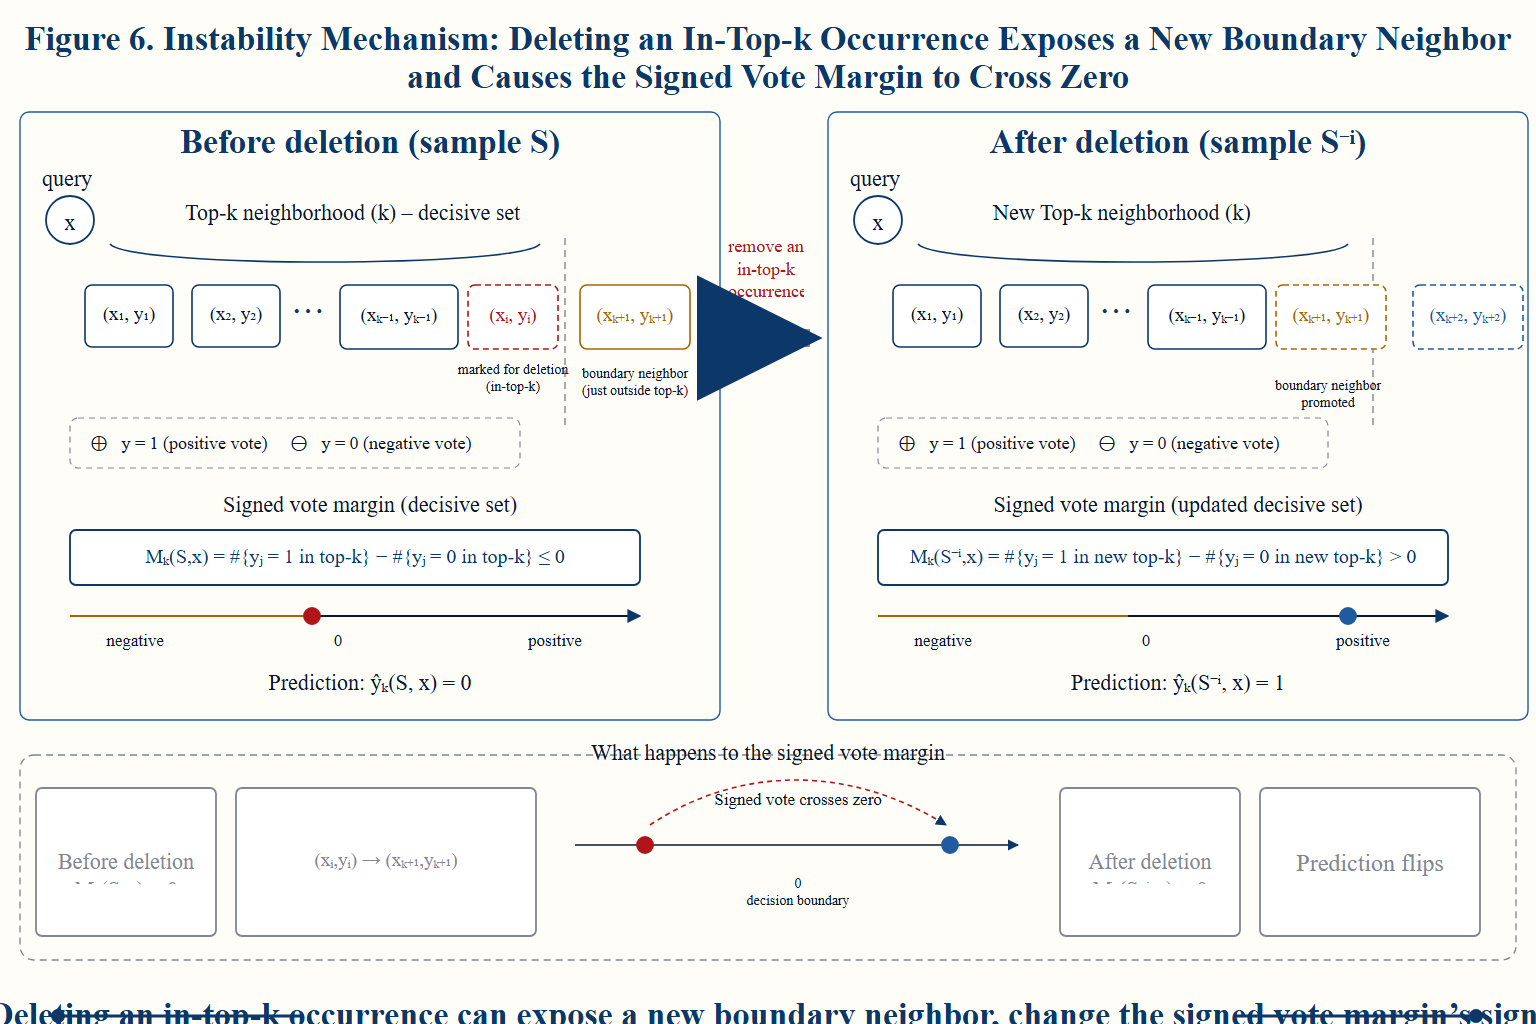
\includegraphics[width=0.82\linewidth]{outputs/figures/recreated_fig06.png}
    \caption{A local perturbation changes the prediction only when the top-$k$
    signed vote crosses zero. This is the exact mechanism behind all explicit
    witnesses in this paper.}
    \label{fig:margin-flip}
\end{figure}

These mechanisms are especially sensitive in the presence of duplicate
occurrences and equal-distance contenders, because the top-$k$ neighborhood is
then controlled by the deterministic tie-breaking convention rather than by
distance alone (\cref{fig:tie-microscope}, \Cref{app:additional-figures}).
This is by design: tie-breaking is part of the object being
studied, not a nuisance to be eliminated.

The rest of the paper uses this margin-based analysis repeatedly. In
the $1$-NN witness of \Cref{sec:finite-separation}, the decisive effect is a
single nearest-occurrence replacement. In the odd-$k$ separation theorem of
\Cref{sec:k-extension}, the construction produces repeated
occurrence patterns whose signed margin is stable under LOO but fragile under a
targeted replace-one move.
